\documentclass[11pt]{article}
\usepackage[margin=2.5cm]{geometry}
\usepackage{amsmath,amssymb,amsthm}
\usepackage{booktabs}
\usepackage{xcolor}
\usepackage{enumitem}
\usepackage{listings}
\usepackage{tikz}
\usetikzlibrary{arrows.meta,positioning,fit,backgrounds}
\usepackage{fancyhdr}
\usepackage[colorlinks=true,linkcolor=blue!50!black,citecolor=blue!50!black,urlcolor=blue!50!black]{hyperref}
\usepackage{parskip}

\definecolor{codebg}{RGB}{245,245,250}
\lstset{basicstyle=\ttfamily\small,backgroundcolor=\color{codebg},breaklines=true,frame=single,columns=fullflexible}

\pagestyle{fancy}
\setlength{\headheight}{14pt}
\fancyhf{}
\lhead{SportsQuant --- Technical Guide}
\rhead{\thepage}
\renewcommand{\headrulewidth}{0.3pt}

\newtheorem{definition}{Definition}

\title{\textbf{SportsQuant}\\[4pt]\large A Statistical Sports-Prediction and Paper-Trading Engine\\[2pt]
\normalsize Models, Data, and the Probability Functions Being Fit}
\author{Prepared for Jes\'us --- built with Claude (Anthropic)}
\date{September 2026}

\begin{document}
\maketitle
\tableofcontents

\section{What this document is}
This is the technical reference for the sports-prediction project: which machine-learning /
statistical models are used, which data trains them, which data is used to produce a prediction
for a specific match, and --- since the request was specifically for ``which probability function
are you trying to fit'' --- the exact functional forms, written out. It also narrates what was
built, in the order it was built, including the parts of an earlier attempt (by Google's
Antigravity agents) that this version replaces and why.

This is a research and paper-trading tool. Nothing in this project places a real bet, logs into a
sportsbook, or should be read as financial advice. Section~\ref{sec:honesty} is the most important
one if you read only one: it lays out exactly which numbers in the app come from a model fitted
on real data, and which come from a placeholder prior, because those are very different things
and the app is designed to never blur them.

\section{One-paragraph summary of how any of this works}
You train a model by giving it many past examples where the outcome is already known (here: past
matches, with the final score) and letting it adjust a small number of parameters --- one or two
numbers per team, plus a handful of shared constants --- until its predicted probabilities are as
consistent as possible with what actually happened, measured by a likelihood function. You then
freeze those parameters and use them to compute a probability for a match whose outcome is not yet
known. Every ``bet'' in the app is a probability read off that fitted model, converted to a fair
decimal price ($1/p$), and compared against a real bookmaker price if you supply one.

\section{System architecture}

\begin{figure}[ht]
\centering
\resizebox{\textwidth}{!}{%
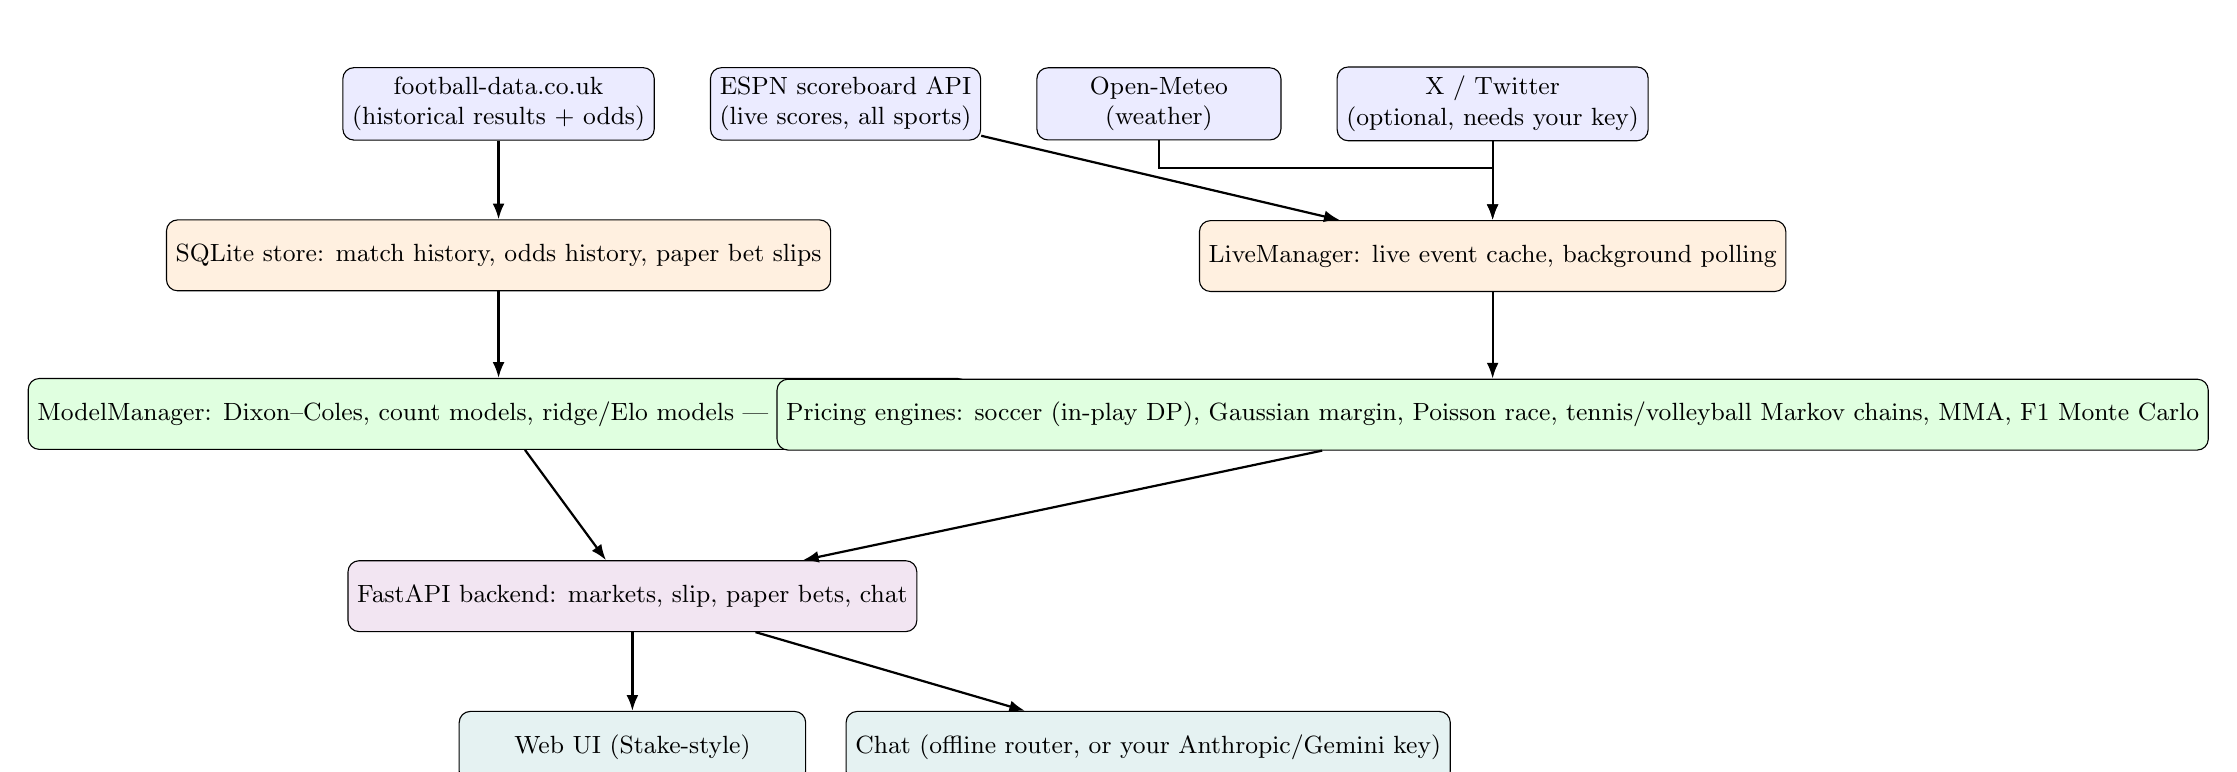
\begin{tikzpicture}[
  box/.style={draw, rounded corners, minimum height=0.9cm, minimum width=3.1cm, align=center, font=\small},
  arr/.style={-{Latex[length=2mm]}, thick},
  node distance=0.6cm and 0.7cm
]
\node[box, fill=blue!8] (fd) {football-data.co.uk\\(historical results + odds)};
\node[box, fill=blue!8, right=of fd] (espn) {ESPN scoreboard API\\(live scores, all sports)};
\node[box, fill=blue!8, right=of espn] (wx) {Open-Meteo\\(weather)};
\node[box, fill=blue!8, right=of wx] (x) {X / Twitter\\(optional, needs your key)};

\node[box, below=1.0cm of fd, fill=orange!12, minimum width=6.6cm] (store) {SQLite store: match history, odds history, paper bet slips};
\node[box, below=1.0cm of x, fill=orange!12, minimum width=6.6cm] (live) {LiveManager: live event cache, background polling};

\node[box, below=1.1cm of store, fill=green!12, minimum width=6.6cm] (models) {ModelManager: Dixon--Coles, count models, ridge/Elo models --- fitted per league};

\node[box, below=1.1cm of live, fill=green!12, minimum width=6.6cm] (engines) {Pricing engines: soccer (in-play DP), Gaussian margin, Poisson race, tennis/volleyball Markov chains, MMA, F1 Monte Carlo};

\node[box, below=1.4cm of models, xshift=1.7cm, fill=violet!10, minimum width=7.2cm] (api) {FastAPI backend: markets, slip, paper bets, chat};

\node[box, below=1.0cm of api, fill=teal!10, minimum width=4.4cm] (ui) {Web UI (Stake-style)};
\node[box, right=0.5cm of ui, fill=teal!10, minimum width=4.4cm] (chat) {Chat (offline router, or your Anthropic/Gemini key)};

\draw[arr] (fd) -- (store);
\draw[arr] (espn) -- (live);
\draw[arr] (wx.south) -- ++(0,-0.35) -| (live.north);
\draw[arr] (x.south) -- ++(0,-0.35) -| (live.north);
\draw[arr] (store) -- (models);
\draw[arr] (live) -- (engines);
\draw[arr] (models) -- (api);
\draw[arr] (engines) -- (api);
\draw[arr] (api) -- (ui);
\draw[arr] (api) -- (chat);
\end{tikzpicture}%
}
\caption{Data flows in from the left (real sources, top row); everything downstream of the
SQLite store and the live cache is this project's own code.}
\end{figure}

Two genuinely different kinds of ``AI'' are at work, and it matters that they are kept separate:

\begin{itemize}
\item \textbf{The prediction models} (Sections~\ref{sec:dixoncoles}--\ref{sec:othersports}) are
classical statistics / maximum-likelihood models, not neural networks and not language models.
They run on a CPU in milliseconds and their entire ``knowledge'' is a few hundred fitted numbers
per league (one attack and one defence strength per team, plus a handful of shared constants).
\item \textbf{The chat} (Section~\ref{sec:chat}) is a large language model (your own Anthropic or
Gemini API key, or a built-in zero-configuration offline keyword router if you supply no key). It
is deliberately never allowed to invent a probability: every number it states comes from calling a
tool that runs the actual statistical model and returns the result as data, which is then just
read back in words. This is enforced in the tool-calling loop
(\texttt{sportsquant/chat/engine.py}), not just requested in a prompt.
\end{itemize}

\section{Data: what trains the model vs.\ what predicts a match}

\begin{table}[h]
\centering
\small
\begin{tabular}{@{}p{4.3cm}p{5.3cm}p{5.6cm}@{}}
\toprule
& \textbf{Used to \emph{train} (fit parameters)} & \textbf{Used to \emph{predict} one match} \\
\midrule
Soccer (Dixon--Coles) &
Full-time and half-time goals for every match in the lookback window (default 3 seasons), per
league, from football-data.co.uk &
The two teams' already-fitted attack/defence numbers, home advantage, and (if unseen) a
name-matching fallback to the league average \\[4pt]
Cards / corners (count model) &
Full-time cards and corners per match, with the referee's name where the source provides it
(England and Scotland files; most European leagues' free files omit it) &
The two teams' fitted ``produces'' / ``concedes'' rates and the named referee's fitted multiplier
\\[4pt]
Basketball / NFL (ridge ratings) &
Historical box scores \emph{once you wire up a results ingester for them} --- see
Section~\ref{sec:honesty}: today this falls back to a same-season win-rate heuristic from ESPN's
own records &
The two teams' rating (or, currently, their season win/loss record) \\[4pt]
Hockey / MLB (Poisson race) &
Same caveat as above &
Same fallback \\[4pt]
Tennis / volleyball &
No historical serve/rally data is ingested yet &
A single externally supplied win-probability estimate is inverted into a serve/rally probability
(Section~\ref{sec:othersports}) \\[4pt]
Live score, clock, injuries, weather &
Never used for training &
Pulled fresh at request time (ESPN, Open-Meteo) and fed into the in-play engine \\
\bottomrule
\end{tabular}
\caption{What is genuinely fitted today is soccer (goals, and cards/corners where the referee is
recorded). Everything else has a working, honestly-labelled placeholder --- see
Section~\ref{sec:honesty}.}
\end{table}

\section{The soccer goals model: Dixon--Coles}
\label{sec:dixoncoles}

\subsection{The probability function being fit}
For a match between home team $i$ and away team $j$, let $(X,Y)$ be the final home and away goal
counts. The model is Dixon and Coles' (1997) modification of the double-Poisson model:
\begin{equation}
P(X=x,\,Y=y)\;=\;\tau_\rho(x,y)\cdot \mathrm{Pois}(x;\lambda_{ij})\cdot \mathrm{Pois}(y;\mu_{ij})
\end{equation}
with scoring rates built from one attack strength $\alpha$ and one defence strength $\delta$ per
team, a shared intercept $c$, and a shared home-advantage term $h$:
\begin{align}
\ln \lambda_{ij} &= c + h + \alpha_i - \delta_j \qquad \text{(home goals)}\\
\ln \mu_{ij} &= c \phantom{{}+h{}} + \alpha_j - \delta_i \qquad \text{(away goals)}
\end{align}
and a low-score correction $\tau_\rho$ that nudges the four cells where goals are 0 or 1 each,
because real 0--0 and 1--1 results are slightly more or less common than two independent Poisson
counts would predict:
\begin{equation}
\tau_\rho(x,y)=
\begin{cases}
1-\lambda\mu\rho & x=0,y=0\\
1+\lambda\rho & x=0,y=1\\
1+\mu\rho & x=1,y=0\\
1-\rho & x=1,y=1\\
1 & \text{otherwise.}
\end{cases}
\end{equation}
$\rho$ is a single number shared by the whole league (typically around $-0.05$ to $-0.10$).
Everything else about the joint scoreline table --- 1X2, over/under, both-teams-to-score, Asian
handicaps, correct score --- is read off this one table $G[x,y]=P(X{=}x,Y{=}y)$ by summing the
right cells; see Section~\ref{sec:markets}.

\subsection{Fitting: the exact objective that is maximised}
Given $N$ historical matches with results $(x_m,y_m)$ played on dates $t_m$, parameters $\theta =
(c,h,\{\alpha_i\},\{\delta_i\},\rho)$ are found by maximising a \emph{weighted, ridge-penalised}
log-likelihood:
\begin{equation}
\mathcal L(\theta) \;=\; \sum_{m=1}^{N} w_m\Big[\ln\tau_\rho(x_m,y_m) + x_m\ln\lambda_m-\lambda_m
+ y_m\ln\mu_m-\mu_m\Big] \;-\; \eta\sum_i\big(\alpha_i^2+\delta_i^2\big)
\end{equation}
where the per-match weight $w_m=\exp(-\xi\cdot\text{age}_m\text{ in days})$ down-weights old
matches ($\xi=0.0019/\text{day}$ by default, an $\approx\!1$-year half-life --- this is the
standard exponential time-decay used in the football-analytics literature, e.g.\ Dixon \& Coles
themselves and later work by Constantinou \& Fenton), and the ridge term with strength $\eta$
shrinks a team's strengths towards the league average when it has few matches (freshly promoted
teams, or teams a league hasn't played this season). Optimisation is L-BFGS-B on the negative
log-likelihood, using an \emph{analytic} gradient (implemented and unit-tested against finite
differences in \texttt{tests/}, not just the numerical optimiser's own internal approximation).

\subsection{How this was validated}
The standard way to check a fitting routine is the same one used for any Monte Carlo or numerical
method in physics: generate synthetic data from a model whose parameters are \emph{known}, fit it,
and confirm the fitted parameters recover the true ones. This project does exactly that
(\texttt{sportsquant/data/synthetic.py} + the test suite): a 20-team, 5-season synthetic league is
simulated by drawing scorelines directly from the Dixon--Coles grid with chosen true
$(\alpha,\delta,h,\rho)$, then fit blind. Over 12 independent random synthetic leagues, the fitted
home-advantage and $\rho$ were unbiased to within $\pm0.01$--$0.04$ of the true value, and the
mean absolute error on each team's attack strength was $\approx\!0.045$ on a scale where true
strengths spanned roughly $\pm0.6$. The analytic gradient matched a finite-difference check to
within $2\times10^{-4}$ over $10^{5}$-scale gradient norms.

\subsection{The card / corner model}
Cards and corners use the same fitting machinery (weighted, ridge-penalised, analytic-gradient
Poisson regression) but with a different, non-symmetric parametrisation, since ``produces cards''
and ``concedes cards'' are conceptually different from ``attacks'' and ``defends'':
\begin{align}
\ln \mathbb E[\text{home count}] &= c + h + f_{\text{home}} - g_{\text{away}} + r_{\text{ref}}\\
\ln \mathbb E[\text{away count}] &= c \phantom{{}+h{}} + f_{\text{away}} - g_{\text{home}} + r_{\text{ref}}
\end{align}
with a Gaussian prior on the referee effect $r$ (shrinking an official with few matches toward
``average referee''), and the predictive distribution is a \emph{negative binomial}, not a
Poisson: $\mathrm{Var} = \mathbb E\,(1+\alpha\,\mathbb E)$, with the extra-spread parameter
$\alpha$ estimated from the Pearson residuals of the fit, because card and corner counts are
empirically over-dispersed relative to a Poisson. \textbf{This model is only as good as the
referee field in the source data}: football-data.co.uk includes it for England and Scotland;
most other free European files do not, in which case the referee term is simply omitted for that
match rather than guessed.

\section{The in-play soccer engine: what actually moves the price after a goal}
\label{sec:inplay}
This is the direct answer to ``does it refresh itself... Barcelona pays 1.25, after they score
twice it goes to 1.04.'' Goals are modelled as two time-inhomogeneous Poisson processes whose
instantaneous rate depends on three things:

\begin{enumerate}[leftmargin=1.4em]
\item \textbf{Time}: expected goals are spread unevenly across the match (a fitted-shape ramp per
half, with $45.5\%$ of a match's goals in the first half by default), not uniformly;
\item \textbf{Score effects}: a team leads by $d$ goals scores at rate $\lambda\cdot e^{-\beta d}$
and the trailing team at $\mu\cdot e^{+\beta d}$ (trailing teams push, leading teams sit back) ---
$\beta=0.08$ here is a literature-typical prior, not yet calibrated on this project's own data;
\item \textbf{Red cards}: a team down a man scores less and concedes more, by fixed multipliers.
\end{enumerate}

Because the rate depends on the \emph{current} score, the distribution of the final score is not a
simple Poisson shift; it is stepped forward minute by minute as a genuine Markov chain (dynamic
programming over the joint count of extra home/away goals). Two properties were checked directly
rather than assumed:
\begin{itemize}
\item With $\beta=0$ and no red cards, the in-play table reduces \emph{exactly} to two independent
Poisson counts over the remaining scoring exposure (checked to $10^{-7}$ against
\texttt{scipy.stats.poisson}) --- the dynamic-programming machinery is not doing anything beyond
what a closed-form calculation would give in the case where it should not be;
\item A \emph{terminal tilt} $R(x,y)=G_{\text{DC}}(x,y)/G_{\text{DP}}(x,y)$ is applied so that at
the exact moment of kickoff the in-play engine's full-match distribution equals the pre-match
Dixon--Coles table \emph{exactly} (checked to $5$ decimal places) --- there is no artificial jump
in the odds the instant the clock starts.
\end{itemize}
The same machinery also prices ``1UP/2UP'' (pays out the moment a team leads by 1 or 2 goals, even
if the match later draws), next-goalscorer timing, and 15-minute goal windows, each solved as an
absorbing/first-passage or hazard calculation on the same minute-by-minute process --- these were
cross-checked against a $20{,}000$-path direct Monte-Carlo simulation of the same process
independently coded, agreeing to within Monte-Carlo noise ($0.7266$ vs.\ $0.7252$ analytically, on
a check with the score-effect switched off so the comparison has a clean interpretation).

\section{Sports other than soccer}
\label{sec:othersports}

\begin{description}
\item[Basketball / NFL --- Gaussian margin model.] A ridge regression on
\emph{margin} (home score $-$ away score) and \emph{total} (sum), each team getting one rating,
solved in closed form (weighted normal equations). In-play, the remaining margin/total is treated
as a Brownian motion: mean drifts by the fitted rate $\times$ time left, variance shrinks $\propto$
time left --- the standard ``win probability from score and time'' construction used throughout
public sports analytics.
\item[Hockey / MLB --- Poisson race.] Same idea as soccer's goal model without the Dixon--Coles
correlation term (rare 0--0/1--1 ties matter less at hockey/baseball scoring rates); ties are
broken with one extra scored event, weighted by a fitted overtime/extra-innings home-side
probability.
\item[Tennis / volleyball --- exact point-by-point Markov chains.] Given a single per-point (or
per-rally) win probability, the \emph{entire} match --- game, set, and match distribution,
including tie-breaks --- is computed exactly by dynamic programming over the point score, memoised
per state (Python \texttt{lru\_cache}), not simulated. Given a desired \emph{match} win
probability, the reverse problem (back out the per-point probability) is solved by one-dimensional
root-finding (Brent's method). Verified: a 60\% server-point-win probability reproduces the
textbook 73.57\% game-win probability exactly; the forward and reverse solves round-trip to 4
decimal places.
\item[MMA / F1.] MMA uses a literature-typical KO/submission/decision method-mix prior applied to
a supplied win probability. F1 runs a $20{,}000$-path Monte Carlo per race: driver rating minus a
grid-penalty term, Gumbel noise (the standard choice for a ``who finishes highest'' ranking model,
equivalent to a softmax over ratings), and an independent per-driver DNF probability.
\end{description}

\section{From a scoreline table to every market on the slip}
\label{sec:markets}
Every market shown --- 1X2, double chance, draw-no-bet, both-teams-to-score, all total-goals
lines, Asian handicaps and Asian totals (including quarter lines, settled as an equal-stake split
across the two neighbouring lines), half-time/full-time, winning margin, correct score, and same-game
combinations --- is computed by summing probability mass over the appropriate cells of the same
joint table $G[x,y]$ (\texttt{sportsquant/markets/scoredist.py}). Same-game parlay legs are priced
by intersecting boolean masks over that table \emph{jointly}, not by multiplying each leg's
marginal probability --- the app explicitly shows the ratio of the true joint probability to the
naive product, because those two numbers are systematically different for correlated legs (e.g.\
``favourite wins'' and ``both teams score'' are negatively correlated: the favourite winning big
and clean-sheeting is a common way for them to win).

\subsection{Odds, edge, and staking --- the definitions used throughout}
\begin{align}
\text{decimal odds } o &: \text{a \$1 stake returns \$}o\text{ in total} \\
\text{implied probability} &= 1/o \\
\text{fair odds for probability } p &= 1/p \\
\text{overround} &= \textstyle\sum_k 1/o_k \;-\;1 \\
\text{edge} &= p\cdot o - 1 \\
\text{Kelly fraction } f^* &= \dfrac{p\cdot o - 1}{o - 1}, \qquad \text{staked at a quarter of }f^*\text{ by default}
\end{align}
Bookmaker margin is removed with Shin's (1993) method by default (also available: proportional,
and the power method), which allocates the overround assuming it partly compensates for
informed/insider money rather than spreading it evenly --- it shades long-shot prices down more
than the proportional method does, which is closer to what is empirically observed in
sharp-book favourite--longshot bias.

\section{What is really fitted, and what is a placeholder --- read this before trusting a number}
\label{sec:honesty}
Every match in the app carries a visible confidence badge, driven directly by the code path that
produced its numbers:

\begin{itemize}
\item \textbf{FITTED MODEL} (green): the two teams were both found in a Dixon--Coles model fit on
real historical results you ingested with \texttt{scripts/ingest.py}.
\item \textbf{LOW-CONFIDENCE PRIOR} (amber): one of three things happened --- (a) a soccer team
wasn't in your ingested history (a promoted team, a league you haven't ingested, a cup tie between
two different leagues), and a league-average prior was used; (b) a non-soccer match is priced from
a same-season ESPN win/loss record via a simple log-odds heuristic, because a proper historical
box-score ingester for that sport is not wired up yet (Section~\ref{sec:roadmap} says exactly what
to build); or (c) no form data was available at all, and a flat league-average prior was used.
\item \textbf{DEMO MODEL} (violet): the match is one of the small set of always-on, clearly-labelled
simulated exhibition matches (Section~\ref{sec:demo}) that keep the app lively between real
kickoffs. Its ``final score'' is a genuine random draw from this project's own in-play engine ---
so watching it is literally watching a sample path of the same model that prices real matches ---
but it is not a real result and never will be.
\end{itemize}
This badge is not cosmetic: it is read directly off the \texttt{confidence} field the pricing
engine returns, the same field the chat is instructed to state alongside any probability.

\section{The demo universe: why matches move even at 3am with nothing real on}
\label{sec:demo}
\texttt{sportsquant/live/providers/sim\_demo.py} keeps a handful of well-known fixtures (e.g.\
Barcelona vs.\ Galatasaray) cycling on a compressed clock (a full ``match'' takes about 8 real
minutes). Each one is a single Monte-Carlo draw from the \emph{same} in-play hazard function
described in Section~\ref{sec:inplay}, revealed minute by minute as the compressed clock advances,
using a seed derived from the fixture name and the current time slot so the same match doesn't
replay identically forever. This is how the ``Barcelona shortens from 1.25 to 1.04 after two
goals'' behaviour can be seen within minutes of starting the app, without waiting for a real
kickoff --- and it is the same code path real matches use, so it is a genuine, honest
demonstration of the engine rather than a scripted animation.

\section{Live data and automatic refresh}
A background thread polls ESPN's public (unofficial, undocumented) scoreboard JSON for every
configured league every \texttt{poll\_live\_seconds} (15s by default) for live matches and every
\texttt{poll\_schedule\_seconds} (10 min) for the upcoming schedule, and re-fits every soccer
model every \texttt{refit\_hours} once enough new results have accumulated. Markets are
\emph{not} pre-computed for every match on a timer; they are computed the moment the browser asks
for a given match (a few milliseconds to about 30ms for the busiest soccer match), so the price
you see is always calculated from the current score and clock, not from a stale cache. Open paper
bet slips are checked against finished matches on the same loop and settled automatically once
every leg's market type supports automatic settlement (1X2, handicaps, totals, BTTS, and similar;
markets like same-game combos or minute windows are not auto-settled yet).

\section{The chat}
\label{sec:chat}
With no API key configured, an offline keyword router (\texttt{OfflineChat}) handles common
requests --- match lookups, value-bet scans, parlay pricing, Kelly sizing, de-vigging --- by
calling the exact same Python functions the web UI uses (\texttt{ToolBox}, shared code, not a
re-implementation). With an Anthropic or Gemini key in \texttt{.env}, the same functions are
exposed to the model as tools; the system prompt explicitly forbids the model from stating a
number it did not get from a tool call, and this was verified structurally (not just by prompting)
by mocking both providers' HTTP APIs and confirming the exact JSON the toolbox returned was what
got sent back to the model on the next turn.

\section{The X / Twitter layer, and why it is off by default}
The project brief asked for a layer that reads soccer Twitter, including explicitly-named
banter and parody accounts. \texttt{config/accounts\_twitter.json} sorts accounts into four tiers
(official, credentialed journalists, community/analytics, and banter/parody/unverified); only
Tier 1--2 can ever produce a ``fact'' flag (e.g.\ a confirmed lineup change), and Tier 4 --- which
includes accounts the project brief itself identified as parody, such as parody accounts of a
well-known transfer journalist --- is never used for anything beyond optional sentiment colour,
and \texttt{sportsquant/social/extractor.py} refuses to pass Tier 3/4 posts into fact extraction
even if asked to. This module is real, working code against X's real API v2 endpoints, but it is
\textbf{inactive until you add your own bearer token}: as of when this was written, X's API has no
free tier for reading posts (roughly \$0.005 per post read), so polling even 30 accounts a few
times a day is a real ongoing cost of roughly \$1--2/day and scales up from there --- a decision
you should make deliberately, not one this project makes for you by defaulting it on.

\section{What was tested, and how}
In the spirit of validating a computational model the way one would in physics --- exact limits,
conservation laws, and Monte Carlo cross-checks, not just ``it ran without crashing'':
\begin{itemize}
\item Every probability table produced by \texttt{ScoreDist} and by each sport's engine was
checked to sum to 1 (a discrete probability conservation law) across dozens of scenarios.
\item Dixon--Coles' analytic gradient was checked against finite differences; the fit was checked
for parameter recovery against synthetic data with known truth, across 12 random seeds.
\item The in-play engine's $\beta=0$ limit was checked against closed-form independent Poisson
counts (max abs.\ difference $1.0\times10^{-7}$); its kickoff-instant behaviour was checked to
match the pre-match model exactly after the terminal tilt; its first-passage (``1UP'') calculation
was cross-checked against an independent $20{,}000$-path Monte-Carlo simulation.
\item The tennis Markov chain was checked against the textbook closed-form game-win probability;
the round-trip (probability $\to$ per-point rate $\to$ probability) was checked to close to 4
decimal places.
\item The real ESPN JSON schema was captured live and used as a test fixture after a first attempt
revealed a real bug (the odds block is nested under the \emph{competition}, not the \emph{event}
--- an easy mistake the fixture test caught immediately).
\item The real football-data.co.uk CSV schema (confirmed against its own published column
documentation) was used to build an ingestion parser tolerant of the columns that differ by
league and season.
\item Every FastAPI endpoint was exercised end-to-end (event listing, market pricing, placing and
auto-settling a paper bet, adding/pricing/clearing a same-match parlay, the chat, both LLM
tool-calling loops with mocked HTTP).
\end{itemize}

\section{What this replaces from the first (Antigravity) attempt, and why}
The first pass, built directly by Google Antigravity's agents, got real things right --- a
Dixon--Coles core, a DuckDB store, a tiered Twitter-account concept, a working Streamlit chat --
and you flagged, correctly, that it was incomplete in specific ways: the referee table in
\texttt{tools.py} hard-coded four names with numbers that were not fitted from anything, and the
team list only covered a handful of Premier League sides. This version fixes that class of problem
structurally rather than by adding more hard-coded rows: referee and team numbers now only exist
if they came out of a real fit (Section~\ref{sec:dixoncoles}), and anything that has not been
fitted says so on screen (Section~\ref{sec:honesty}) instead of presenting a guess as if it were
a fact.

\section{Honest limitations}
\begin{itemize}
\item The score-effect strength $\beta$, red-card multipliers, and the weather-to-goals adjustment
are literature-typical priors, not calibrated on this project's own data yet.
\item Basketball, NFL, hockey and MLB do not yet have a historical box-score ingester wired up
(Section~\ref{sec:roadmap}), so they run on a same-season record heuristic until one is added.
\item Referee and card/corner modelling is only as complete as the source data: most non-English
free files do not include a referee column.
\item The market is usually at least as well-informed as this model, and often more so. A fitted
model and a positive expected value calculation are not a guarantee of anything; they are an
estimate with real uncertainty around it. Treat the value-finder and Kelly-sizing tools as a
paper-trading and closing-line-value research exercise, not a source of income, and re-read
Section~\ref{sec:markets}'s point about correlated parlay legs before trusting a multi-leg number
someone else's app gave you without that correction.
\end{itemize}

\section{Suggested next steps}
\label{sec:roadmap}
\begin{enumerate}
\item Run \texttt{scripts/ingest.py --all} for real Big-5-plus-extras history, then watch the
confidence badges on real fixtures turn from amber to green.
\item Wire up a historical results ingester for basketball/NFL/hockey/MLB (the same
\texttt{Store.add\_result} table already exists; \texttt{ModelManager.refit} already fits a
\texttt{MarginModel} the moment enough rows exist for a competition) --- see
\texttt{prompts/06\_other\_sports\_ingestion.md}.
\item Calibrate $\beta$, the red-card multipliers, and the weather adjustment against your own
ingested results instead of the literature priors currently in \texttt{InPlayParams}.
\item Only if you decide the cost is worth it: add an X bearer token and build out
\texttt{extract\_flags}'s LLM prompt for real injury/lineup extraction, then feed confirmed flags
into the pre-match rate as an explicit multiplier with its own fitted effect size, the same way
the referee effect is fitted today --- not as a hard-coded adjustment.
\end{enumerate}

\end{document}
